\documentclass{article}
\usepackage{times}
\usepackage[spanish, activeacute]{babel}
\usepackage{graphicx}
\usepackage[utf8]{inputenc}
\usepackage[colorlinks=true,linkcolor=blue,urlcolor=blue]{hyperref} 
\pagestyle{empty}
\setlength{\textheight}{8.75in}
\setlength{\columnsep}{2.0pc}
\setlength{\textwidth}{6.8in}
\setlength{\topmargin}{0.25in}
\setlength{\headheight}{0.0in}
\setlength{\headsep}{0.0in}
\setlength{\oddsidemargin}{-.19in}
\setlength{\parindent}{1pc}
\makeatletter
\def\@normalsize{\@setsize\normalsize{12pt}\xpt\@xpt
\abovedisplayskip 10pt plus2pt minus5pt\belowdisplayskip \abovedisplayskip
\abovedisplayshortskip \z@ plus3pt\belowdisplayshortskip 6pt plus3pt
minus3pt\let\@listi\@listI} 
\def\subsize{\@setsize\subsize{12pt}\xipt\@xipt}
\def\section{\@startsection {section}{1}{\z@}{24pt plus 2pt minus 2pt}
{12pt plus 2pt minus 2pt}{\large\bf}}
\def\subsection{\@startsection {subsection}{2}{\z@}{12pt plus 2pt minus 2pt}
{12pt plus 2pt minus 2pt}{\subsize\bf}}
\makeatother
\usepackage{listings}
\usepackage{xcolor}

\definecolor{codegreen}{rgb}{0,0.6,0}
\definecolor{codegray}{rgb}{0.5,0.5,0.5}
\definecolor{codepurple}{rgb}{0.58,0,0.82}
\definecolor{backcolour}{rgb}{0.95,0.95,0.92}

\lstdefinestyle{mystyle}{
   % backgroundcolor=\color{backcolour},   
    commentstyle=\color{codegreen},
    keywordstyle=\color{magenta},
    numberstyle=\tiny\color{codegray},
    stringstyle=\color{codepurple},
    basicstyle=\ttfamily\footnotesize,
    breakatwhitespace=false,         
    breaklines=true,                 
    captionpos=b,                    
    keepspaces=true,                 
    numbers=left,                    
    numbersep=5pt,                  
    showspaces=false,                
    showstringspaces=false,
    showtabs=false,                  
    tabsize=2
}
\lstset{style=mystyle}


\begin{document}
\date{}

%Colocar el nombre del reporte
\title{\Large\bf Proyecto Final de Probabilidad y Procesos Estocásticos.}

%colocar el nombre del autor o autores, asi como la universidad y departamento
\author{ Jairo Cain Sanchez Estrada \\ 
\\
  M. en C. en Ingeniería Electrónica y Computación\\
  Control automático \\ 
  Centro Universitario de Ciencias Exactas e Ingenierías\\
  Universidad de Guadalajara}

\maketitle
\thispagestyle{empty}

%Aqui se escribe el abstract
%----------------------------------------------------------------------------------------
\subsection*{\centering Abstract}
\textit{Este documento comprende el trabajo final correspondiente a la asignatura de Probabilidad y procesos estocásticos de la Maestría en Ciencias en Ingeniería Electrónica y Computación en el ciclo 2014B.}
%----------------------------------------------------------------------------------------

%Aqui va la introduccion. En el primer renglon se escribe una cita a una referencia
%----------------------------------------------------------------------------------------
\section{Introducción}\label{sec:intro}
El procesamiento digital de imágenes es un campo de investigación abierto \cite{femat1999}. El constante progreso en esta área no ha sido por sí mismo, sino en conjunto con otras áreas con las cuales esta relacionada como las matemáticas, la computación, y el conocimiento cada vez mayor de ciertos órganos del cuerpo humano que intervienen en la percepción y en la manipulación de las imágenes. Aunado a esto, la inquietud del hombre por imitar y usar ciertas características del ser humano como apoyo en la solución de problemas. El avance del Procesamiento Digital de Imágenes se ve reflejado en la medicina, la astronomía, geología, microscopía, etc. Información meteorológica, transmisión y despliegue agilizado de imágenes por Internet tienen sustento gracias a estos avances.
El término "imagen monocromática" o imagen simplemente, se refiere a una función de intensidad de luz bidimensional $f(x,y)$, donde $x$ e $y$ indican las coordenadas espaciales y el valor de $f$ en cualquier punto $(x,y)$ es proporcional a la luminosidad (o nivel de gris) de la imagen en dicho punto.
Una imagen digital es una imagen (función) $f(x,y)$ que ha sido discretizada tanto en coordenadas espaciales como en luminosidad.
%----------------------------------------------------------------------------------------



%Aqui va el desarollo de la practica
%----------------------------------------------------------------------------------------
\section{Desarrollo}\label{sec:desarr}
El histograma de una imagen digital con valores de gris dentro del rango [0, $L-1$] es una función discreta $h(r_{k})=n_{k}$, donde $r_{k}$ es el $k$-ésimo nivel de gris y $n_{k}$ es el número de pixeles de la imagen que tienen el nivel de gris $r_{k}$.
Es práctica común normalizar el histograma dividiendo cada uno de sus valores por el número total de pixeles en la imagen, denotado como $n$, como sigue: $p(r_{k})=n_{k}/n$.
En términos generales, $p(r_{k})$ es un estimado de la probabilidad de ocurrencias del nivel de gris $r_{k}$. La suma de todos los componentes de un histograma normalizado es $= 1$.
Las imágenes cuyos pixeles tienden a ocupar el rango dinámico entero de posibles valores de niveles de gris, y además, tienden a estar distribuídos de manera uniforme, tendrán una apariencia de mejor contraste y exhibirán una gran variedad de tonos de gris. 
Los niveles de gris de una imagen pueden ser vistos como una variable aleatoria en el intervalo de [0,1]. Uno de los descriptores fundamentales de las variables aleatorias es la función de densidad de probabilidades.
Para valores discretos trabajamos con probabilidades y sumatorias en lugar de funciones de densidad de probabilidad e integrales. La probabilidad de la ocurrencia de un nivel de gris $r_{k}$ en una imagen se aproxima como:


%---------------De esta forma se pueden declarar ecuaciones-----------
%----------------------------------------------------------------------------------------
\begin{equation}
P_{r}(r_{k})=\frac{n_{k}}{n} \qquad k=0,1,2,...,L-1
\label{eq:1} 
\end{equation}
%----------------------------------------------------------------------------------------

donde $n$ es el número total de pixeles de la imagen, $n_{k}$ es el número de pixeles que tienen el nivel de gris $r_{k}$, y $L$ es el número total de posibles niveles de gris en la imagen.

La versión discreta de la función de transformación (es decir, de la función de distribución acumulada) es:

\begin{equation}
S_{k}=T(r_{k})=\sum \limits_{j=0}^{k}P_{r}(r_{j})
\label{eq:1} 
\end{equation}

\begin{equation}
S_{k}=\sum \limits_{j=0}^{k} \frac{n_{j}}{n} \qquad k=0,1,2,...,L-1
\label{eq:1} 
\end{equation}

La imagen procesada (salida) se obtiene mapeando cada pixel con valor $r_{k}$ de la imagen de entrada a su correspondiente nivel $s_{k}$ en la imagen de salida. A esta transformación se le llama ecualización del histograma o linearización del histograma. 

La ecualización del histograma determina automáticamente la función de transformación y busca 
producir una imagen de salida que tenga un histograma uniforme. El método es simple deimplementar.La ecualización del histograma determina automáticamente la función de transformación y busca producir una imagen de salida que tenga un histograma uniforme. El método es simple de implementar.\\

Sin embargo, existen aplicaciones en las que intentar producir histogramas uniformes no siempre es la mejor opción. En particular, es útil algunas veces tratar de especificar la forma del histograma de la imagen de salida, a esta técnica se le conoce como especificación del 
histograma (\emph{histogram matching}).\\

Suponga los niveles de gris continuos $r$ y $z$ (variables aleatorias continuas), y sea $p_{r}(r)$ y $p_{z}(z)$ sus correspondientes funciones de densidad de probabilidad. $r$ y $z$ denotan los niveles de gris de la imagen de entrada y de salida respectivamente.\\

Se puede estimar $p_{r}(r)$ de la imagen de entrada, y $p_{z}(z)$ es la función de densidad de probabilidad especificada que deseamos que tenga la imagen de salida.\\

Sea $s$ una variable aleatoria discreta que define una transformación:

\begin{equation}
s_{k}=T(r_{k})=\sum \limits_{j=0}^{k} p_{r}(r_{j})
\end{equation}

\begin{equation}
S_{k}=\sum \limits_{j=0}^{k} \frac{n_{j}}{n} \qquad k=0,1,2,...,L-1
\end{equation}

donde $n$ es el número total de pixeles de la imagen, $n_{j}$ es el número de pixeles que tienen el nivel de gris $r_{j}$, y L es el número total de posibles niveles de gris en la imagen. Reconocemos esta ecuación como la ecualización del histograma.\\

Del histograma especificado $p_{z}(z_{i})$, $i=0, 1, 2, …, L-1$ se obtiene la función de transformación $G(z)$:

\begin{equation}
v_{k}=G(z_{k})=\sum \limits_{i=0}^{k} p_{z}(z_{i})=s_{k} \qquad k=0,1,2,...,L-1
\end{equation}

Estamos buscando valores de $z$ que satisfagan esta ecuación. De las dos últimas expresiones sigue que $G(z)=T(r)$. La variable $v_{k}$ se añadió por claridad con la discusión que sigue.\\

Obtener la función de transformación inversa $G^{-1}$:

\begin{equation}
z_{k}=G^{-1}[T(r_{k})] \qquad k=0,1,2,...,L-1
\end{equation}

\begin{equation}
z_{k}=G^{-1}(s_{k}) \qquad k=0,1,2,...,L-1
\end{equation}

Las ecuaciones 4 y 5  son el mapeo de los niveles de gris de la imagen original a los correspondientes niveles $s_{k}$ basados en el histograma de la imagen original. La ecuación 6 calcula la función de transformación G del histograma especificado $p_{z}(z)$ dado. Y finalmente, las ecuaciones 7 y 8 nos dan una aproximación de los niveles deseados de la imagen con ese histograma.
%----------------------------------------------------------------------------------------

%Aqui va la seccion de resultados
%----------------------------------------------------------------------------------------
\section{Resultados}\label{sec:res}
Los resultados son obtenidos mediante un programa que busca la correcta ecualización de una imagen por dos métodos:

\begin{itemize}
\item Ecualización del histograma por medio de una función de densidad
\item Ecualización del histograma por medio de una función de densidad especificada
\end{itemize}
%----------------------------------------------------------------------------------------

%Aqui se pone el codigo 
%----------------------------------------------------------------------------------------
\subsection{Código en C}\label{sec:cod}
\textbf{Nota:} El programa fue reducido en algunas de sus líneas por motivos de espacio en el \emph{template}. El archivo fue previamente enviado mediante un correo al profesor junto con una copia de este reporte.\\

%Aqui se llama al archhivo o archivos que tienen su codigo
\lstinputlisting[language=c]{./codigo/arreglo.c}
%----------------------------------------------------------------------------------------


%Aqui hay ejemplos de como incoluir imagenes
%----------------------------------------------------------------------------------------
\subsection{Imágenes resultantes}\label{sec:ima}
En esta subsección se presentan las imágenes resultantes de los métodos de ecualización por una función de densidad y por una función de densidad especificada. Cada una de las imágenes resultantes, al igual que la imagen original, vienen acompañadas por su histograma, histograma normalizado e histograma acumulado normalizado.

Como se puede apreciar en la Fig. \ref{fig:2}, nuestra imagen original es una imagen cuyos valores se encuentran claramente en el dominio de las bajas intensidades (esto en referencia a la escala de grises). Esta observación es corroborada en mediante el histograma de la imagen (Fig. \ref{fig:2}).

\begin{figure}
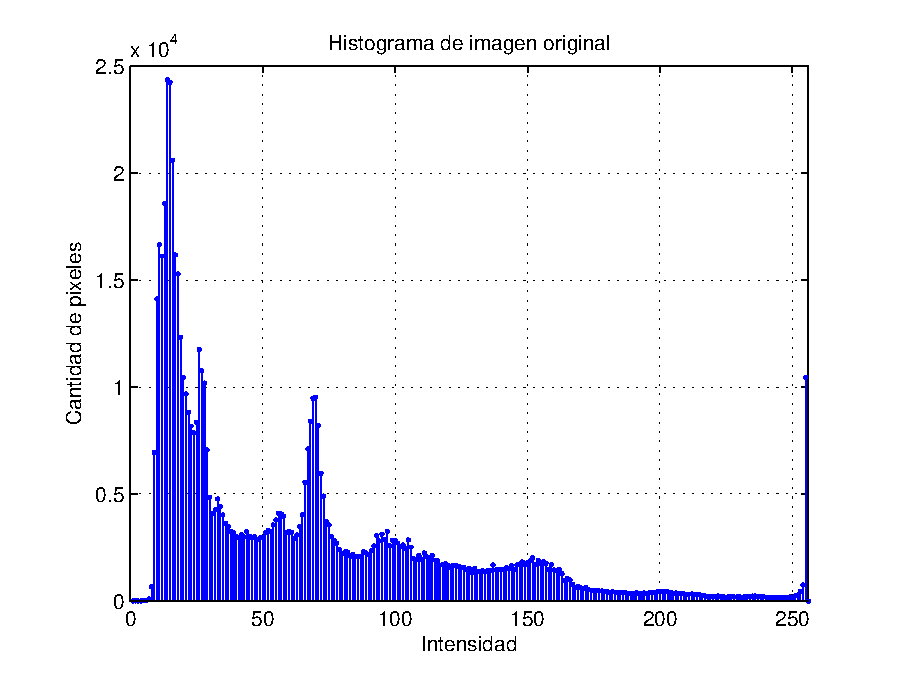
\includegraphics[width=1\textwidth]{imagen/imagen002.eps}
\caption{Histograma acumulado normalizado de imagen ecualizada por referencia.}
\label{fig:2} 
\end{figure}
%----------------------------------------------------------------------------------------

%Aqui van las conclusiones
%----------------------------------------------------------------------------------------
\section{Conclusiones}\label{sec:con}
Pese a conseguir una mejor distribución en el dominio de las intensidades de la imagen, el método de ecualización del histograma por medio de una función de densidad muestra cambios abruptos en la imagen. En cambio, el método de ecualización de la imagen por medio de una función especificada, muestra variaciones más suaves. Sin embargo, la distribución del dominio de las intensidades de la imagen es mayor en el método de ecualización del histograma por medio de una función de densidad. 
%----------------------------------------------------------------------------------------

\bibliographystyle{IEEEtran}
\bibliography{biblio}
\end{document}
